\chapter{Introduction}
This work is concerned with the issues of emulating different loads using power electronic converters. The scope of the problem as follows:
\begin{itemize}
\item To implement models of machine type loads.
\item Study issues of modelling machine type loads under faulted condition.
\item Study issues of modelling solid-state loads (thyristor converter).
\end{itemize}
In developing motion control systems it is common
practice to employ simulators to experiment with proposed designs and their effect on the performance of the system. These simulators are typically implemented
on a digital computer using a high-level language program to solve a system of differential equations in a time-stepping fashion. \par
Due to the lack of 
accurate mathematical models of many physical systems, experiments cannot be completely
eliminated in real-time. In an effort to fill in the gap between digital simulations in a computer and final
experiments on the product, Hardware In- the Loop (HIL) has become a widely adopted technique.
HIL typically refers to a system where some of the hardware or mechanical devices are replaced by
controllers interfacing in real-time with sensors and actuators ~\cite{peter}. With a HIL system, one can finish most of the design and test iterations in a highly efficient highly flexible environment, as long as the HIL is an adequately realistic representation of the actual plant. The fidelity of the HIL system depends on
how well it emulates the dynamics of the replaced components or subsystems. This is the motivation
of dynamic load emulation. However in this research work a different  approach is proposed for real-time load emulation using HIL system. The system  uses the real controller running in its own processor, but rather than a real load  connected to the converter, the controller acts on a simulation of load model  and draws required currents of the actual system from the source.\par 
 For example, manufacturers of inverters will normally test prototype and preproduction equipment with a standard induction motor. This, motor may not always have the desired characteristics for a particular test, or may  not be well matched to the intended application. The
same arguments apply for generation applications which utilize power electronic conversion equipment. It is also the case that, in some testing situations, the manufacturer may wish to include characteristics of the mechanical load or prime mover. For instance, when
testing an electric vehicle drive inverter, it would be useful to load the inverter with something which represents the characteristics of the vehicle during particular driving conditions. Similarly, a machine tool manufacturer may wish to test electric drive inverters with loads which characterize the dynamics, duty cycles and work piece variations of the machine tool. With these arrangements, long-term thermal tests can be carried out under realistic conditions. A similar benefit could be obtained in a generation application, for instance, in a variable speed wind generation system. Here, the generator is producing power in accordance with a randomly varying wind source. This subjects the power converter to randomly varying conditions, which are difficult to replicate in a test laboratory.\par
\begin{figure}[ht]
\centering
\scalebox{0.5}{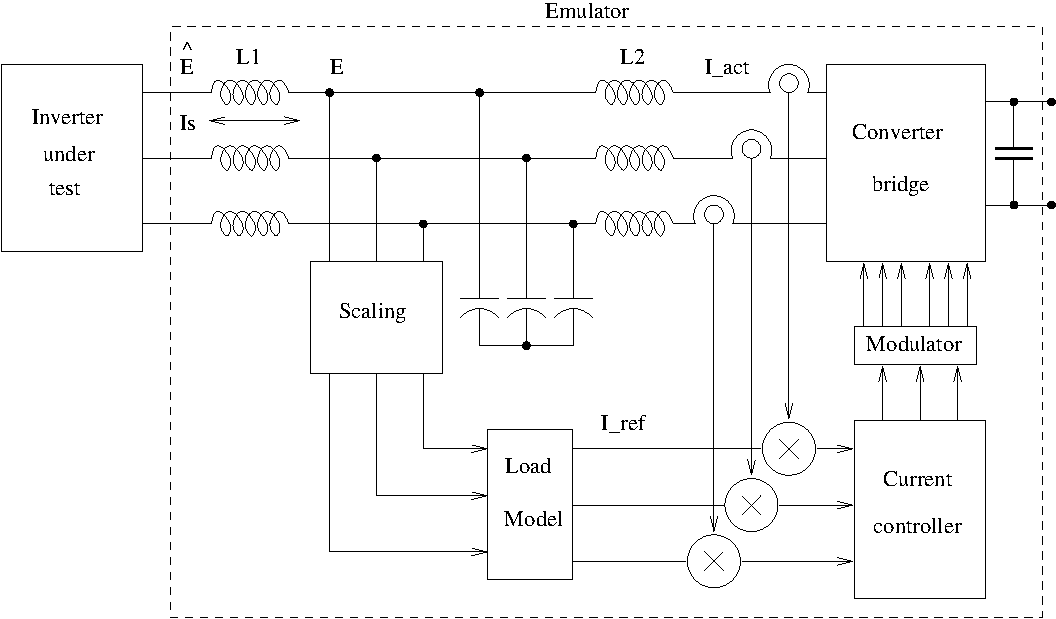
\includegraphics{vmb.pdf}}
\caption{Load Emulation block diagram.}
\label{vmb}
\end{figure}
This report presents a new idea to overcome the above testing difficulties in the form of a `virtual load'. The load emulation is composed of a bidirectional power converter, real-time digital system and a closed loop control system. The real time system is described below  produce a programmable load/source, which can be connected directly to the power electronic inverter as a replacement for an electrical load. There may be some confusion between the inverter and the converters which form the virtual load, as shown in Fig. \ref{vmb} `inverter' will be taken to mean the inverter being tested and `converter' will be used to describe the power electronics in the virtual load. The virtual load is effectively a power level active impedance. It is important to realize that the virtual load is
capable of bidirectional power flow and also transient and steady-state operation. These features allow it to emulate the characteristics of a wide range of electrical machines and their associated mechanical loads. The complexity of the emulation is limited only by the
capability of the bidirectional power converter and the real-time simulation which controls it.\par
Bidirectional power converters are now commonplace. The special feature of the converter used for the emulation role is that it must act at least as fast as the inverter being tested. A priori the assumption might be that the converter needs to be very fast, and that this
might threaten the viability of the idea. In practice, the converter is used in conjunction with energy storage (i.e. inductors), which effectively slow changes down and reduce the bandwidth required.\par
\section{Motivation}
This work was motivated by the need to emulate the loads which allows the user to test both the hardware and the software of the inverter. The virtual load can provide different load characteristics with which the control algorithms and inverter design can be
tested. The flexibility of the load emulation allows the designer of the control algorithms to experiment with different designs safe in the knowledge that if something goes wrong expensive damage to the inverter and machine will not result. A rotating machine cannot be stopped instantly: it has inertia. The load emulation contains no rotating parts, it is made up of fast acting power electronics which can handle a fault situation and prevent unnecessary damage.\par
The load emulation system has regeneration capability, as the power flow from the inverter can be returned to the mains supply. When testing an inverter with an actual machine, the machine uses this power for rotation and it is therefore lost. As well as being a small energy benefit this also reduces the laboratory power supply requirements.
\section{Objectives}
\begin{itemize}
\item To study various Real-time simulation methods.
\item To study various current control methods.
\item Detailed simulation of current controllers such as:
1. Synchronous reference PI regulator.
2. Hysteresis current controller.
3. Dead-beat current controller. 
\item To investigate the issues involved in the use of power electronic converter to emulate electrical loads.
\item Design and implementation of experimental setup for virtual load emulation.
\item Analysis, simulation and laboratory implementation of `virtual Machine' in steady state as well in transient condition.
\item Study issues of modelling machine loads under faulted condition.
\item Study issues of modelling solid-state loads (thyristor converter).
\item To study and simulation of interface impedance for various load models.
\item To study and simulation of bidirectional power flow for AC to AC converter.
\end{itemize}
\section{Layout of the Report} A brief chapter by chapter overview is presented here.\\
Chapter 2: A literature review of different real-time simulation methods for load emulation is presented.  \\
Chapter 3: Experimental setup, digital signal processor system, inverter, PWM generation will be described in this chapter.\\
Chapter 4: In this chapter, the most essential information on dynamical system model, Reference frame theory and basic equations for virtual machine are presented.  \\
Chapter 5: Survey on current control methods are presented in this chapter. Investigation on the basic performance of current controller will be made using circuit simulation software SEQUEL. The results obtained from simulation are discussed.\\
Chapter 6: Some of the important design issues will be highlighted in this chapter. Being a non-ideal device, the inverter has many drawbacks. Dead-time between the IGBT switching, resistive voltage drop of the switching components and the DC-link voltage fluctuations have been identified as the most problematic non-idealizes. Analysis of the adverse effects of these problems and compensation methods will be the focus of this chapter.\\
Chapter 7:  The problem of ripple output at the inverter legs and bidirectional power flow  will be the focus of this chapter.\\
Chapter 8: Conclusions and discussion on future course of research work.\\
